\section{Local rates and stalling near a minimizer}\label{sec:local-rates}

This section quantifies items (ii) and (iii) of
Section~\ref{sec:three-limits} near a global minimizer $x^*$. It answers
three questions. How fast do the iterates contract? How large is their
limit as a function of the cutoff slack $\epsilon=U-f^*$? When do fixed
boxes exist at every small scale, so that no number of rounds tightens
anything? The answers depend on the relaxation family through a
second-order \emph{tangent model}, the limit of the relaxation rescaled to
boxes that shrink to $x^*$, and on an associated map on box shapes. They
take the form of sufficient conditions for geometric contraction and for
stalling; Example~\ref{ex:critical-scalar} shows that a valid monotone
family can satisfy neither.

Throughout, $U=f^*+\epsilon$ with $\epsilon\ge0$, and the order hypotheses
of Section~\ref{sec:foundations} hold on all boxes used, including the
comparison boxes $x^*+tD(d)$ introduced below. By
Lemmas~\ref{lem:sequential} and~\ref{lem:fixed-persist}, the upper bounds
on widths and rates below hold for Jacobi rounds and for complete
sequential rounds, the stall statements hold for every update scheme, and
lower bounds and exact rates are statements about Jacobi rounds. All
results involve $x^*$, $f^*$, and tangent data that a solver does not know.
Their role is to identify which limit dominates and how it scales;
Section~\ref{sec:certificates} supplies computable certificates.

\subsection{Two scalar bounds}\label{sec:local-rates-scalar}

The simplest estimates compare the relaxation with a growth function of
the distance to $x^*$. They fix two regimes.

\begin{proposition}[Sharp growth]\label{prop:sharp-growth}
Suppose $\kappa>0$ and $\tau\ge0$ satisfy
\begin{equation}\label{eq:sharp-growth}
  \phi_B(x)\ge f^*+\kappa\norm{x-x^*}_\infty-\tau w(B)^2
\end{equation}
for every box $B$ with $x^*\in B\subseteq B_0$ and every $x\in B$. Then
\[
  w(T_U(B))\le\frac{2}{\kappa}\bigl(\epsilon+\tau w(B)^2\bigr)
\]
for every such box. Suppose some iterate satisfies $w(B_K)\le\kappa/(4\tau)$
(any iterate if $\tau=0$). If $\epsilon=0$, then
$w(B_{k+1})\le(2\tau/\kappa)w(B_k)^2$ for $k\ge K$ and $B_\infty=\{x^*\}$.
If $\epsilon>0$, then $w(B_{k+1})\le w(B_k)/2+2\epsilon/\kappa$ for $k\ge K$
and $w(B_\infty)\le4\epsilon/\kappa$.
\end{proposition}

\begin{proof}
A point $x\in K_U(B)$ satisfies
$\kappa\norm{x-x^*}_\infty\le\phi_B(x)-f^*+\tau w(B)^2\le\epsilon+\tau w(B)^2$,
and every coordinate range of $K_U(B)$ is at most twice this radius. If
$w(B_k)\le\kappa/(4\tau)$, then $(2\tau/\kappa)w(B_k)^2\le w(B_k)/2$; since
the iterates are nested, all later iterates stay in this region. Hence
$w(B_{k+1})\le w(B_k)/2+2\epsilon/\kappa$ for $k\ge K$, and the limit of the
nonincreasing widths is at most $4\epsilon/\kappa$. For $\epsilon=0$ the
widths tend to zero, the quadratic recurrence holds, and $x^*\in B_k$ for
every $k$.
\end{proof}

The one-round bound is the mechanism of marginals-based range reduction:
a relaxation whose value grows at least linearly with slope $\kappa$ away
from a bound cannot keep points farther than $(U-L)/\kappa$ from that
bound~\cite{ryoo1995-global-optimization-of-nonconvex-nlps}. Condition~\eqref{eq:sharp-growth} is a
statement about all relaxed points, not only feasible ones. It holds, for
example, in a problem with only bound constraints whose objective satisfies
$f(x)-f^*\ge\kappa\norm{x-x^*}_\infty$ on $B_0$ and whose relaxation
satisfies $\phi_B\ge f-\tau w(B)^2$ on $B$. It also holds on small boxes at a
vertex minimizer at which every partial derivative is nonzero and makes the
objective increase into the box (strict complementarity in every
coordinate), for the composite relaxations of
Section~\ref{sec:local-rates-factorable}: on boxes containing such a vertex
the first-order term is at least $\kappa\norm{x-x^*}_\infty$ with $\kappa$
the smallest absolute partial derivative, and Theorem~\ref{thm:composite-expansion}
bounds the rest by a multiple of $w(B)^2$.

\begin{proposition}[Quadratic growth]\label{prop:quadratic-growth}
Suppose $\mu>0$ and $\tau\ge0$ satisfy
\[
  \phi_B(x)\ge f^*+\mu\norm{x-x^*}_\infty^2-\tau w(B)^2
\]
for every box $B$ with $x^*\in B\subseteq B_0$ and every $x\in B$. Then
$w(T_U(B))^2\le4\epsilon/\mu+q^2w(B)^2$ with $q^2=4\tau/\mu$. If $q<1$, the
iterates satisfy
\[
  w(B_k)^2\le q^{2k}w(B_0)^2+\frac{4\epsilon}{\mu}\,\frac{1-q^{2k}}{1-q^2},
  \qquad
  w(B_\infty)\le2\sqrt{\frac{\epsilon}{\mu-4\tau}},
\]
and for $\epsilon=0$ the widths contract at least by the factor $q$ per
round.
\end{proposition}

\begin{proof}
A point of $K_U(B)$ lies within $\infty$-norm distance
$\sqrt{(\epsilon+\tau w(B)^2)/\mu}$ of $x^*$. Bound each coordinate range by
twice this radius, square, and iterate the affine recurrence for
$w(B_k)^2$.
\end{proof}

For $\epsilon>0$ the proposition bounds the widths by a scalar envelope; it
does not assert that the distance to the actual limit box contracts by the
factor $q$. The strict condition $\tau<\mu/4$ has the same numerical
threshold as conditions excluding the cluster problem in branch and bound: with
$\mu=\lambda_1/2$, where $\lambda_1$ is the smallest eigenvalue of the
Hessian at $x^*$, the threshold is $\lambda_1/8$, compared with
$K\le\lambda_1/8$ in Wechsung,
Schaber, and Barton~\cite{wechsung2014-the-cluster-problem-revisited}, and
with $\mu=\gamma/2$ it is $\gamma/8$, compared with
$\tau^*\le\gamma/8$ in Kannan and
Barton~\cite{kannan2017-the-cluster-problem-in-constrained}. Their
prefactors bound the gap between minimum values; here $\tau$ bounds the
pointwise gap over the box, which is at least as large. Both bounds are far
from necessary. For $f(x,y)=x^2+y^2+xy$ with the McCormick envelope of $xy$,
the best constants are $\mu=3/4$ (on the face $x=1$ of the unit cube the
minimum of $f$ is attained at $y=-1/2$) and $\tau=1/4$, so $q^2=4/3>1$, yet
Jacobi rounds contract by the factor $0.7247$
(Proposition~\ref{prop:two-variable-rate}). The scalar bound charges the
largest relaxation gap at every point and the weakest growth in every
direction. The tangent model keeps the dependence on the shape of the box
and on the position inside it.

\subsection{The tangent model and the tangent map}\label{sec:local-rates-tangent}

A \emph{shape} is a vector $d=(d^-,d^+)\in\R^{2n}_{\ge0}$, and
$D(d)=\prod_{i=1}^n[-d_i^-,d_i^+]$. Every box containing $x^*$ can be written
as $x^*+tD(d)$ with $t>0$. For a shape $u\gg0$, meaning that all $2n$
components are positive, the \emph{gauge} of a box $B=[\ell,u']\ni x^*$ is
\[
  g_u(B)=\min\{t\ge0:B\subseteq x^*+tD(u)\}
  =\max_i\max\Bigl\{\frac{x_i^*-\ell_i}{u_i^-},\frac{u'_i-x_i^*}{u_i^+}\Bigr\}.
\]
The endpoint vector of $x^*+tD(d)$ is $p(\{x^*\})+td$; shapes are endpoint
vectors measured from $x^*$.

\begin{assumption}[Tangent model]\label{ass:tangent}
The point $x^*\in X\cap B_0$ is a global minimizer, and there is a function
$Q(d,\xi)\in\R$, defined for shapes $d$ and $\xi\in D(d)$, with the following
property. For every compact set $\mathcal K$ of shapes there is $t_{\mathcal K}>0$
such that the boxes $x^*+tD(d)$, $d\in\mathcal K$, $0<t\le t_{\mathcal K}$,
belong to $\mathfrak B$ and
\begin{equation}\label{eq:tangent}
  \varrho_{\mathcal K}(t)=\sup_{d\in\mathcal K,\ \xi\in D(d)}
  \frac{\bigl|\phi_{x^*+tD(d)}(x^*+t\xi)-f^*-t^2Q(d,\xi)\bigr|}{t^2}
  \longrightarrow0\qquad(t\downarrow0).
\end{equation}
\end{assumption}

The function $Q$ is the \emph{tangent model} of the relaxation family at
$x^*$. Assumption~\ref{ass:tangent} requires finite relaxation values on
the comparison boxes and no first-order term, so it describes interior
minimizers and minimizers on faces at which the objective has zero
derivative across the face. For quadratic objectives with McCormick
relaxations the remainder in~\eqref{eq:tangent} is zero
(Section~\ref{sec:local-rates-quadratic}); for composite McCormick
relaxations of factorable functions, $Q$ is computed by a recursion over
the factors (Theorem~\ref{thm:composite-expansion}). Minimizers on the
boundary with nonzero derivatives are treated in
Section~\ref{sec:local-rates-boundary}. The restricted tangent contraction for
exactly represented linear equations closes
Section~\ref{sec:local-rates-contraction}.

For $c\ge0$ and a shape $d$, let
\[
  S_c(d)=\{\xi\in D(d):Q(d,\xi)\le c\},
\]
and define the shape $\Phi_c(d)\in\R^{2n}_{\ge0}$ by
$\hull S_c(d)=D(\Phi_c(d))$, that is, $\Phi_c(d)_i^-=-\min_{\xi\in S_c(d)}\xi_i$
and $\Phi_c(d)_i^+=\max_{\xi\in S_c(d)}\xi_i$. The \emph{tangent map} is
$\Phi=\Phi_0$. In scaled coordinates, $\Phi$ describes one Jacobi round on a
box $x^*+tD(d)$ at zero cutoff slack, up to the remainder
in~\eqref{eq:tangent}.

\begin{lemma}[Properties of the tangent model]\label{lem:tangent-properties}
Under Assumption~\ref{ass:tangent}:
\begin{enumerate}[label=(\alph*)]
\item $Q(sd,s\xi)=s^2Q(d,\xi)$ for $s>0$;
\item if $d\le d'$, then $Q(d,\xi)\ge Q(d',\xi)$ for $\xi\in D(d)$;
\item $Q(d,0)\le0$;
\item $Q(d,\cdot)$ is lower semicontinuous on $D(d)$, and convex if every
  $\phi_B$ is convex;
\item $S_c(d)$ is compact and contains $0$, so $\Phi_c(d)$ is well defined;
  moreover $\Phi_c(d)\le d$, $\Phi_c(d)\le\Phi_c(d')$ if $d\le d'$,
  $\Phi_c(d)\le\Phi_{c'}(d)$ if $c\le c'$, and
  $\Phi_c(sd)=s\Phi_{c/s^2}(d)$; in particular $\Phi$ is order preserving
  and positively homogeneous of degree one;
\item $\Phi_c(d)\to\Phi(d)$ componentwise as $c\downarrow0$.
\end{enumerate}
\end{lemma}

\begin{proof}
(a) The box $x^*+tD(sd)$ equals $x^*+(ts)D(d)$, and the point $x^*+t(s\xi)$
equals $x^*+(ts)\xi$. Apply~\eqref{eq:tangent} with
$\mathcal K=\{d,sd\}$ to both descriptions, divide by $t^2$, and let
$t\downarrow0$. (b) For $d\le d'$ the box $x^*+tD(d)$ is contained in
$x^*+tD(d')$; apply monotonicity at $x^*+t\xi$, subtract $f^*$, divide by
$t^2$, and let $t\downarrow0$. (c) Validity at the feasible point $x^*$
gives $\phi_B(x^*)\le f^*$. (d) For fixed $d$, $Q(d,\cdot)$ is the uniform
limit on $D(d)$ of the real-valued functions
$\xi\mapsto t^{-2}(\phi_{x^*+tD(d)}(x^*+t\xi)-f^*)$, which are lower
semicontinuous, and convex if $\phi_B$ is. Uniform limits of lower
semicontinuous functions are lower semicontinuous, and pointwise limits
of convex functions are convex. (e) Compactness follows from (d), and
$0\in S_c(d)$ from (c). The inclusion $S_c(d)\subseteq D(d)$ gives
$\Phi_c(d)\le d$; for $d\le d'$, (b) gives $S_c(d)\subseteq S_c(d')$; and
$S_c(d)$ increases with $c$. By (a),
$\xi\in S_c(sd)$ if and only if $\xi/s\in S_{c/s^2}(d)$, so
$S_c(sd)=sS_{c/s^2}(d)$. (f) The sets $S_c(d)$ are compact, decrease as
$c\downarrow0$, and have intersection $S_0(d)$. For a fixed component,
choose a maximizer $\xi^c$ of $\xi_i$ over $S_c(d)$; every cluster point
of $\xi^c$ as $c\downarrow0$ lies in $S_0(d)$, so the maxima converge to the
maximum over $S_0(d)$. Minima are analogous.
\end{proof}

The following constant measures contraction. It is an upper
Collatz--Wielandt number of the order-preserving homogeneous map $\Phi$,
made robust to a small cutoff slack.

\begin{definition}[Contraction factor of the tangent map]
\[
  r^*=\inf\{\lambda\ge0:\ \Phi_\delta(u)\le\lambda u\text{ for some }u\gg0
  \text{ and some }\delta>0\}.
\]
\end{definition}

\begin{lemma}\label{lem:cw}
Under Assumption~\ref{ass:tangent}, $0\le r^*\le1$ and
$r^*=\inf\{\lambda\ge0:\ \Phi(u)\le\lambda u\text{ for some }u\gg0\}$.
\end{lemma}

\begin{proof}
$\Phi_\delta(u)\le u$ gives $r^*\le1$. Since $\Phi\le\Phi_\delta$, the right
side is at most $r^*$. Conversely, if $\Phi(u)\le\lambda u$ with $u\gg0$ and
$\lambda'>\lambda$, then $\lambda u<\lambda'u$ componentwise, and
Lemma~\ref{lem:tangent-properties}(f) gives $\Phi_\delta(u)\le\lambda'u$ for
small $\delta>0$; hence $r^*\le\lambda'$.
\end{proof}

If the remainder in~\eqref{eq:tangent} is zero and $\epsilon=0$, a Jacobi
round maps $x^*+tD(d)$ exactly to $x^*+tD(\Phi(d))$, so the exact asymptotic
rate is the growth rate of $\Phi^k(d)$. This rate never exceeds $r^*$:
if $\Phi(u)\le\lambda u$ and $d\le su$, then $\Phi^k(d)\le s\lambda^ku$.
Proposition~\ref{prop:tangent-eigenrate} proves equality when $\Phi$ has a
positive eigenvector. Equality in general would require further properties
of $\Phi$, such as continuity, which we do not establish; we use $r^*$ only
as an upper bound.

\subsection{Contraction, exact rates, and stalling}\label{sec:local-rates-contraction}

\begin{theorem}[Local contraction]\label{thm:tangent-contraction}
Let Assumption~\ref{ass:tangent} hold, and let $u\gg0$, $\delta>0$, and
$\lambda\in(0,1)$ satisfy $\Phi_\delta(u)\le\lambda u$. There is $\bar t>0$
with the following properties.
\begin{enumerate}[label=(\alph*)]
\item If $B$ is a box with $x^*\in B$ and $g_u(B)=t\le\bar t$, and
  $t^2\ge2\epsilon/\delta$, then $g_u(T_U(B))\le\lambda t$.
\item If $g_u(B_0)\le\bar t$, the Jacobi iterates, and the iterates of
  complete sequential rounds, satisfy
  \[
    g_u(B_k)\le\max\bigl\{\lambda^kg_u(B_0),\ \sqrt{2\epsilon/\delta}\bigr\},
    \qquad B_\infty\subseteq x^*+\sqrt{2\epsilon/\delta}\,D(u).
  \]
  In particular, for $\epsilon=0$ the iterates converge to $\{x^*\}$ and
  $g_u(B_k)\le\lambda^kg_u(B_0)$.
\end{enumerate}
\end{theorem}

\begin{proof}
Choose $\bar t\le t_{\{u\}}$ such that $\varrho_{\{u\}}(t)\le\delta/2$ for
$t\le\bar t$. (a) If $t=0$, then $B=\{x^*\}$ and there is nothing to prove.
Otherwise let $C=x^*+tD(u)$, so that $B\subseteq C$. A point
$x=x^*+t\xi\in K_U(C)$ satisfies
\[
  t^2Q(u,\xi)-\tfrac{\delta}{2}t^2\le\phi_C(x)-f^*\le\epsilon\le\tfrac{\delta}{2}t^2,
\]
so $Q(u,\xi)\le\delta$ and $\xi\in S_\delta(u)$. Hence
$T_U(C)\subseteq x^*+tD(\Phi_\delta(u))\subseteq x^*+\lambda tD(u)$, and
$T_U(B)\subseteq T_U(C)$ by Lemma~\ref{lem:order}. (b) The gauges of the
nested iterates are nonincreasing. If $g_u(B_k)\ge\sqrt{2\epsilon/\delta}$,
part (a) gives $g_u(B_{k+1})\le\lambda g_u(B_k)$; otherwise
$g_u(B_{k+1})\le g_u(B_k)<\sqrt{2\epsilon/\delta}$. Induction gives the
displayed bound, and $B_\infty\subseteq B_k$ gives the inclusion. Complete
sequential rounds are covered by Lemma~\ref{lem:sequential}.
\end{proof}

\begin{corollary}[Rate and floor]\label{cor:tangent-rate}
Suppose Assumption~\ref{ass:tangent} holds and $r^*<1$. For every
$\lambda\in(r^*,1)$ there are $u\gg0$, $\delta>0$, and $\bar t>0$ such that
the conclusions of Theorem~\ref{thm:tangent-contraction} hold for every
start box $B_0\ni x^*$ with $w(B_0)\le\bar t\min_ju_j$. For $\epsilon=0$ the
iterates converge to $x^*$ linearly with factor $\lambda$ in the gauge
$g_u$. For $\epsilon>0$,
$w(B_\infty)\le\sqrt{2\epsilon/\delta}\,\max_i(u_i^-+u_i^+)$. If moreover
$X\cap B_0$ contains a neighborhood of $x^*$ on which
$f\le f^*+M\norm{x-x^*}_\infty^2$ for some $M>0$, then
$w(B_\infty)\ge2\sqrt{\epsilon/M}$ for small $\epsilon$, so under these
additional premises the width of the limit is of order exactly
$\sqrt\epsilon$.
\end{corollary}

\begin{proof}
By the definition of $r^*$ there are $u\gg0$, $\delta>0$, and
$\lambda'<\lambda$ with $\Phi_\delta(u)\le\lambda'u\le\lambda u$. A box
containing $x^*$ with width at most $\bar t\min_ju_j$ has gauge at most
$\bar t$. The upper bound on $w(B_\infty)$ is
Theorem~\ref{thm:tangent-contraction}(b). For the lower bound, every point
of the cube $x^*+\sqrt{\epsilon/M}\,[-1,1]^n$ is feasible for small
$\epsilon$ and has objective at most $U$, so the cube lies in $H_U$, which
lies in $B_\infty$ by Lemma~\ref{lem:sublevel-hull}.
\end{proof}

The upper bound on the rate is exact in the presence of an eigenvector.

\begin{proposition}[Exact rate from a positive eigenvector]\label{prop:tangent-eigenrate}
Suppose the tangent model is exact,
$\phi_{x^*+tD(d)}(x^*+t\xi)=f^*+t^2Q(d,\xi)$ for all $t>0$ and all shapes
$d$ for which the box belongs to $\mathfrak B$, and let $\epsilon=0$. If
$\Phi(u)=\rho u$ for some $u\gg0$, then
$T_U^k(x^*+tD(u))=x^*+\rho^ktD(u)$ and $r^*=\rho$. If the Jacobi iterates
start from a box with $x^*+aD(u)\subseteq B_0\subseteq x^*+bD(u)$, $a>0$, and
all these comparison boxes belong to $\mathfrak B$, then
\[
  x^*+a\rho^kD(u)\subseteq B_k\subseteq x^*+b\rho^kD(u).
\]
Hence, if $\rho>0$, $w(B_k)=\Theta(\rho^k)$ and $w(B_k)^{1/k}\to\rho$; if
$\rho=0$, then $B_1=\{x^*\}$.
\end{proposition}

\begin{proof}
With zero remainder and $\epsilon=0$, $K_U(x^*+tD(d))=x^*+tS_0(d)$, so
$T_U(x^*+tD(d))=x^*+tD(\Phi(d))$, and induction proves the first identity.
Monotonicity of $T_U$ gives the sandwich. For $r^*$, Lemma~\ref{lem:cw}
gives $r^*\le\rho$. If $\Phi(v)\le\lambda v$ for some $v\gg0$ and
$\lambda<\rho$, choose $a>0$ with $au\le v$; then
$a\rho^ku=\Phi^k(au)\le\Phi^k(v)\le\lambda^kv$ for all $k$, which is
impossible. Lemma~\ref{lem:cw} then gives $r^*\ge\rho$.
\end{proof}

The lower bound uses Jacobi rounds; sequential rounds can be strictly
faster, as the example after Lemma~\ref{lem:sequential} shows exactly.

We now give a sufficient condition for fixed boxes to exist at every
sufficiently small scale.

\begin{theorem}[Stalling]\label{thm:local-stall}
Let Assumption~\ref{ass:tangent} hold. Let $v$ be a nonzero shape and
$\delta>0$, and suppose that for every positive component $v_i^+$ there is
$\xi\in D(v)$ with $\xi_i=v_i^+$ and $Q(v,\xi)\le-\delta$, and likewise for
every positive component $v_i^-$ with $\xi_i=-v_i^-$. Then there is
$\bar t>0$ such that $x^*+tD(v)$ is a fixed box of $T_U$ for every
$t\in(0,\bar t]$ and every $U\ge f^*$. Every Jacobi, sequential, or selective
iteration started from a box containing $x^*+\bar tD(v)$, with cutoffs at
least $f^*$, keeps this box; in particular
$w(B_k)\ge\bar t\max_i(v_i^-+v_i^+)$ for all $k$, whatever $\epsilon\ge0$.
Moreover $r^*=1$.
\end{theorem}

\begin{proof}
Choose $\bar t$ with $\varrho_{\{v\}}(t)<\delta$ for $t\le\bar t$. For a
witness $\xi$ as in the hypothesis,
$\phi_{x^*+tD(v)}(x^*+t\xi)<f^*+t^2(-\delta+\delta)=f^*\le U$, so
$x^*+t\xi\in K_U(x^*+tD(v))$. A component of $v$ that is zero needs no
witness: the face then passes through $x^*$, which lies in $K_U$ by
validity. Thus every face of $x^*+tD(v)$ is attained, and the box is fixed.
Lemma~\ref{lem:fixed-persist} gives the persistence. For $r^*$, the same
witnesses lie in $S_0(v)$, so $\Phi(v)=v$. If $\Phi(u)\le\lambda u$ with
$u\gg0$ and $\lambda<1$, choose $s$ with $v\le su$; then
$v=\Phi^k(v)\le s\lambda^ku\to0$, a contradiction. Lemma~\ref{lem:cw} gives
$r^*=1$.
\end{proof}

Under the hypotheses of Theorem~\ref{thm:local-stall}, the limit box does
not shrink to $x^*$ as $\epsilon\downarrow0$. Improving the incumbent cannot
remove the fixed boxes $x^*+tD(v)$ or force convergence to $x^*$, although
it can still remove parts of a larger box outside them; the obstruction is
the relaxation, not the near-optimal set. With zero remainder, the same
proof needs only $Q(v,\xi)\le0$ at the witnesses
(Proposition~\ref{prop:quadratic-rows}). With a nonzero remainder the strict
margin $\delta$ is needed; Example~\ref{ex:critical-scalar} has tangent
witnesses with value zero and no positive-width fixed box.

Both theorems are governed by the values of $Q$ on the faces of a shape.
For a shape $d$ and a component $d_i^+>0$, define the face value
$m_i^+(d)=\min\{Q(d,\xi):\xi\in D(d),\ \xi_i=d_i^+\}$, and $m_i^-(d)$
analogously; the minima exist by Lemma~\ref{lem:tangent-properties}(d).

\begin{corollary}[Face test]\label{cor:face-test}
Let Assumption~\ref{ass:tangent} hold and let $d$ be a nonzero shape.
\begin{enumerate}[label=(\alph*)]
\item If $d\gg0$ and every face value of $d$ is positive, then for every
  $\delta$ with $0<\delta<\min_{i,\pm}m_i^\pm(d)$ there is $\lambda<1$ with
  $\Phi_\delta(d)\le\lambda d$; hence $r^*<1$ and
  Theorem~\ref{thm:tangent-contraction} applies with $u=d$.
\item If every face value of $d$ for a positive component is negative, then
  Theorem~\ref{thm:local-stall} applies with $v=d$.
\end{enumerate}
If every $\phi_B$ is convex, each face value is a convex program, and $2n$
convex programs evaluate both tests at a given shape. The tests are
sufficient conditions; zero or mixed signs leave the question open.
\end{corollary}

\begin{proof}
(a) If $\Phi_\delta(d)_i^+=d_i^+$, a maximizer $\xi$ of $\xi_i$ over $S_\delta(d)$
has $\xi_i=d_i^+$ and $Q(d,\xi)\le\delta<m_i^+(d)$, which contradicts the
definition of $m_i^+(d)$. Hence every component of $\Phi_\delta(d)$ is
strictly smaller than the corresponding component of $d$, and
$\lambda=\max_{i,\pm}\Phi_\delta(d)_i^\pm/d_i^\pm<1$. (b) The minimizers
defining the face values are the witnesses of Theorem~\ref{thm:local-stall}.
\end{proof}

When the signs of the face values are mixed, a tangent round at zero cutoff
slack, that is, one application of $\Phi$, moves the endpoints with positive
face value and keeps the others; the shape changes, and the test must be
repeated on the new shape. Example~\ref{ex:shape-change} shows that the same
objective can stall on one shape and tighten on another. For relaxations
with a nonzero remainder, strict signs give the same conclusion on
sufficiently small boxes at zero cutoff slack, whereas a positive slack can
keep a face whose tangent value is positive. The next example shows that
the two sufficient conditions do not exhaust the possibilities.

\begin{example}[A critical tangent map]\label{ex:critical-scalar}
Let $n=1$, $X=\R$, $f(x)=x^2$, $B_0=[-1/2,1/2]$, and for every subbox $B$
\[
  \phi_B(x)=x^2-E(w(B)),\qquad E(w)=\frac{w^2}{4}-\frac{w^3}{8}.
\]
On $[0,1]$, $E\ge0$ and $E'(w)=w/2-3w^2/8\ge0$, so the family is valid,
convex, continuous, and monotone. At $U=f^*=0$ the cutoff set of a box of
width $w>0$ lies in an interval of width $2\sqrt{E(w)}=w\sqrt{1-w/2}<w$, so no
box of positive width is fixed. On $tD(d)$, with $s=d^-+d^+$,
$\phi(t\xi)=t^2(\xi^2-s^2/4)+t^3s^3/8$, so Assumption~\ref{ass:tangent} holds
with $Q(d,\xi)=\xi^2-s^2/4$ and a remainder of order $t^3$. For $c\ge0$,
$\Phi_c(d)=(\min\{d^-,q\},\min\{d^+,q\})$ with $q=(s^2/4+c)^{1/2}\ge s/2$,
so $\Phi_c$ keeps the smaller component of every shape and $r^*=1$. The face
values of $d=(1,1)$ are zero, so neither test applies. The iteration is
neither stalled nor geometric. From $[-h_0,h_0]$ with $0<h_0\le1/2$, the
Jacobi radii satisfy $h_{k+1}=h_k\sqrt{1-h_k}$; they decrease to zero and
\[
  \frac1{h_{k+1}}-\frac1{h_k}=\frac{1}{\sqrt{1-h_k}\,(1+\sqrt{1-h_k})}\to\frac12,
\]
so $h_k\sim2/k$. At a cutoff slack $\epsilon\in(0,h_0^3)$ the radii follow
$h_{k+1}=\min\{h_k,g(h_k)\}$ with $g(h)=(\epsilon+h^2-h^3)^{1/2}$. The function
$g$ is increasing on $(0,1/2]$, $g(\epsilon^{1/3})=\epsilon^{1/3}$, and
$\epsilon^{1/3}<g(h)<h$ for $h>\epsilon^{1/3}$, so the radii decrease to
$\epsilon^{1/3}$ and the limit has width $2\epsilon^{1/3}$, larger than any
$O(\sqrt\epsilon)$ bound for small $\epsilon$. Finally, the actual face
values $\phi_{[-t,t]}(\pm t)=t^3$ are positive although the tangent face
values vanish, which is why Theorem~\ref{thm:local-stall} requires a strict
margin.
\end{example}

\begin{remark}[Linear equations kept exactly]\label{rem:linear-equations}
A projected relaxation that keeps an affine equality exactly is infinite off
the feasible affine set, so Assumption~\ref{ass:tangent} must be restricted
to that set. The following proposition gives the contraction result;
Proposition~\ref{prop:equality-con} in Section~\ref{sec:equality-con}
computes one exact constrained map.
\end{remark}

Let the feasible
set be $X=\{x:Cx=c_0\}$, intersected with the box $B_0$, and let the
relaxation on $B$ be
\[
 \phi_B(x)=\phi_B^0(x)\ \text{if }Cx=c_0,\qquad
 \phi_B(x)=+\infty\ \text{otherwise},
\]
where $\phi_B^0$ is a valid and monotone relaxation of $f$ that is finite
on $B$. This construction is valid and monotone because the equality does
not depend on $B$. We use the shapes $D(u)$ and the gauge $g_u$ defined above.

\begin{proposition}[Restricted tangent contraction]\label{prop:restricted-tangent-con}
Let $x^*$ lie in the interior of $B_0$ and minimize $f$ on $X\cap B_0$,
let $f$ be differentiable at $x^*$, and let $U=f^*+\epsilon$ with
$\epsilon\ge0$. Fix a shape $u\gg0$ and suppose
that the boxes $x^*+tD(u)$ belong to $\mathfrak B$ for small $t>0$ and
that a function $Q(u,\cdot)$ on $N_u=D(u)\cap\ker C$ satisfies
\[
 \sup_{\xi\in N_u}\frac{\bigl|\phi^0_{x^*+tD(u)}(x^*+t\xi)-f^*
  -t\nabla f(x^*)^T\xi-t^2Q(u,\xi)\bigr|}{t^2}\longrightarrow0
 \qquad(t\downarrow0).
\]
Let $S^C_\delta(u)=\{\xi\in N_u:Q(u,\xi)\le\delta\}$ and define the shape
$\Phi^C_\delta(u)$ by $\hull S^C_\delta(u)=D(\Phi^C_\delta(u))$. If
$\delta>0$ and $\lambda\in(0,1)$ satisfy $\Phi^C_\delta(u)\le\lambda u$,
there is $\bar t>0$ with the following properties.
\begin{enumerate}
\item[(a)] If $B\ni x^*$ has $g_u(B)=t\le\bar t$ and
 $t^2\ge2\epsilon/\delta$, then $g_u(T_U(B))\le\lambda t$.
\item[(b)] If $g_u(B_0')\le\bar t$, the Jacobi iterates from $B_0'$, and the
 iterates of complete sequential rounds, satisfy
 $g_u(B_k)\le\max\{\lambda^kg_u(B_0'),\sqrt{2\epsilon/\delta}\}$; at zero
 cutoff slack they converge to $x^*$ with one-round factor at most
 $\lambda$ in the gauge $g_u$.
\end{enumerate}
\end{proposition}

\begin{proof}
For $\xi\in\ker C$ and small $s>0$, the points $x^*\pm s\xi$ are feasible,
so minimality gives $\nabla f(x^*)^T\xi=0$; the first-order term vanishes
on $N_u$. Taking $\xi=0$ in the expansion and using validity,
$\phi^0_B(x^*)\le f^*$, gives $Q(u,0)\le0$, so $S^C_\delta(u)$ contains
$0$. Choose $\bar t$ such that $x^*+\bar tD(u)\subseteq B_0$ and the
remainder is at most $\delta t^2/2$ on $N_u$ for $t\le\bar t$.
(a) If $t=0$, then $B=\{x^*\}$, and validity gives $T_U(B)=\{x^*\}$.
Otherwise $t>0$; put $B'=x^*+tD(u)\supseteq B$. Lemma~\ref{lem:order} gives
$T_U(B)\subseteq T_U(B')$. A point of $K_U(B')$ has the form $x^*+t\xi$
with $\xi\in D(u)$ and $C\xi=0$, and
$f^*+t^2Q(u,\xi)-\delta t^2/2\le\phi_{B'}(x^*+t\xi)\le f^*+\epsilon$.
Hence $Q(u,\xi)\le\epsilon/t^2+\delta/2\le\delta$, so every retained
$\xi$ lies in $S^C_\delta(u)$, and
$T_U(B')\subseteq x^*+tD(\Phi^C_\delta(u))\subseteq x^*+\lambda tD(u)$.
Thus $g_u(T_U(B))\le\lambda t$. (b) Validity keeps $x^*$ in every iterate,
so the gauges are defined and, by nesting, nonincreasing. Apply (a) while
$g_u(B_k)\ge\sqrt{2\epsilon/\delta}$; below that value nesting keeps
$g_u(B_{k+1})\le g_u(B_k)$. Complete sequential rounds end inside the
Jacobi image by Lemma~\ref{lem:sequential}(b).
\end{proof}

The proposition is the constrained counterpart of
Theorem~\ref{thm:tangent-contraction}, with the tangent support problems
restricted to the nullspace of $C$. The first-order term of the expansion
need not vanish on the whole space; minimality on the affine set removes
it on the nullspace. In Proposition~\ref{prop:equality-con}, $x^*=0$, the expansion has zero
remainder, and $Q(\mathbf 1,(\xi_1,-\xi_1))=2\xi_1^2+4|\xi_1|-2$ on the
unit cube shape $\mathbf 1$. Its zero sublevel set on the nullspace is
$|\xi_1|\le\sqrt2-1$, so $\Phi^C_0(\mathbf 1)=(\sqrt2-1)\mathbf 1$ is an
eigenvector shape, and the factor $\sqrt2-1$ of
Proposition~\ref{prop:equality-con}(a) is attained exactly. The
proposition is conditional on a restricted expansion that is uniform on
the nullspace and on a strict contraction of the restricted map. Nonlinear
equality constraints cannot simply be replaced by their first-order
tangent spaces: the curvature of the constraint and the remainder on
finite boxes must be controlled. Section~\ref{sec:repair-con} obtains such control from a feasible repair.

\subsection{Quadratic objectives with McCormick relaxations}\label{sec:local-rates-quadratic}

Let
\[
  f(x)=f^*+\tfrac12(x-x^*)^TH(x-x^*)
\]
with $H$ symmetric and $H_{ii}\ge0$, and let the relaxation keep the
diagonal terms exactly and replace each off-diagonal term
$H_{ij}(x_i-x_i^*)(x_j-x_j^*)$, $i<j$, by $H_{ij}$ times the McCormick
underestimator of the product if $H_{ij}>0$ and the overestimator if
$H_{ij}<0$. McCormick planes commute with translation: the translation
$x=x^*+y$ adds the same affine function to every plane, so maxima and minima
of planes commute with it. The relaxation is therefore the one a solver
builds for $f$ written in the original variables. The planes also scale
quadratically, so the tangent model is exact:
\begin{equation}\label{eq:quadratic-Q}
  \phi_{x^*+tD(d)}(x^*+t\xi)=f^*+t^2Q(d,\xi),\qquad
  Q(d,\xi)=\sum_i\frac{H_{ii}}{2}\xi_i^2+\sum_{i<j}H_{ij}\,m_{ij}^d(\xi),
\end{equation}
where $m_{ij}^d$ is the McCormick estimator of $\xi_i\xi_j$ over $D(d)$ of
the sign just described. On the unit cube $D(1)=[-1,1]^n$, with
$s_{ij}=\sgn H_{ij}$,
\begin{equation}\label{eq:cube-Q}
  Q(1,\xi)=\sum_i\frac{H_{ii}}{2}\xi_i^2
  +\sum_{i<j}\abs{H_{ij}}\bigl(\abs{\xi_i+s_{ij}\xi_j}-1\bigr).
\end{equation}
A centered box with half-widths $h_i$ reduces to the unit cube by the
substitution $\xi_i=h_i\eta_i$, which replaces $H$ by
$H'=\operatorname{diag}(h)H\operatorname{diag}(h)$, because the McCormick
estimator of $\xi_i\xi_j$ on the box is $h_ih_j$ times the estimator of
$\eta_i\eta_j$ on the cube. If $H_{ii}<0$, a convex relaxation uses the chord
$\frac{H_{ii}}{2}\bigl((d_i^+-d_i^-)\xi_i+d_i^-d_i^+\bigr)$ of the concave
term; the model is still exact but different, and we do not consider this
case. If $X\supseteq B_0$, an interior global minimizer forces $H$ to be
positive semidefinite; an indefinite $H$ requires constraints that exclude
its directions of negative curvature from the local feasible set, for
example linear equations kept exactly as in
Remark~\ref{rem:linear-equations}.

\begin{proposition}[Two variables]\label{prop:two-variable-rate}
Let $f(x,y)=x^2+y^2+axy$ with $0<\abs a<2$, and let $U=f^*=0$. On every
centered cube, a Jacobi round multiplies the half-width by
\[
  \rho(a)=\frac{\sqrt{2a^2+4\abs a}-\abs a}{2}.
\]
The function $\rho$ increases with $\abs a$ from $0$ to $1$; for example
$\rho(0.5)=0.5406$, $\rho(1)=0.7247$, $\rho(1.5)=0.8702$, and
$\rho(1.9)=0.9748$. Every box containing $0$ in its interior has Jacobi
iterates with $w(B_k)=\Theta(\rho(a)^k)$, and $r^*=\rho(a)$. For
$f=\alpha x^2+\beta y^2+cxy$ with $\alpha,\beta>0$ and
$\abs c<2\sqrt{\alpha\beta}$, the same holds with $a=c/\sqrt{\alpha\beta}$,
and the boxes with $\sqrt\alpha\,h_x=\sqrt\beta\,h_y$ play the role of the
cubes.
\end{proposition}

\begin{proof}
Let $a>0$. On $[-1,1]^2$ the underestimator of $xy$ is $\abs{x+y}-1$, so
$Q(1,\xi)=\xi_1^2+\xi_2^2+a(\abs{\xi_1+\xi_2}-1)$. Fix $\xi_1=t\ge0$ and
write $s=\xi_1+\xi_2$. Minimizing $t^2+(s-t)^2+a\abs s-a$ over $s$ gives the
minimizer $s=0$ for $t\le a/2$ and $s=t-a/2$ for $t\ge a/2$, with values
\[
  m_a(t)=2t^2-a\quad(0\le t\le a/2),\qquad
  m_a(t)=t^2+at-\tfrac{a^2}{4}-a\quad(t\ge a/2).
\]
The minimizing $\xi_2$ is $-t$ or $-a/2$, which lies in $[-1,1]$. The function
$m_a$ is continuous and increasing for $t>0$, so the largest $t$ with
$m_a(t)\le0$ is the positive root of the second expression, $\rho(a)$; the
second expression applies because $\rho(a)>a/2$, which is equivalent to
$a<2$, and $\rho(a)\le1$ because $a^2\le4$. The symmetries
$(\xi_1,\xi_2)\mapsto(\xi_2,\xi_1)$ and $\xi\mapsto-\xi$ preserve the cube and
$Q(1,\cdot)$, so $\Phi(1)=\rho(a)1$. The derivative of $\rho$ is positive
because $(2a+2)^2>2a^2+4a$. For $a<0$, the reflection
$\xi_2\mapsto-\xi_2$ preserves the cube and turns the overestimator
term $\abs a(\abs{\xi_1-\xi_2}-1)$ into $\abs a(\abs{\xi_1+\xi_2}-1)$.

The relaxation is defined and monotone on all boxes of $\R^2$, so the
comparison cubes may extend beyond $B_0$. A box containing $0$ in its
interior lies between two centered cubes, and
Proposition~\ref{prop:tangent-eigenrate} gives the rate and $r^*$. For the
last claim, the substitution $z_1=\sqrt\alpha\,x$, $z_2=\sqrt\beta\,y$ maps
the objective to $z_1^2+z_2^2+(c/\sqrt{\alpha\beta})z_1z_2$, and McCormick
estimators commute with positive scaling of the variables.
\end{proof}

The proposition proves $w(B_k)=\Theta(\rho^k)$ from every interior box; it
does not prove that the successive width ratios converge from arbitrary
boxes. The tangent map on other shapes is also explicit.

\begin{proposition}[Centered rectangles]\label{prop:rectangle-map}
Let $f=x^2+y^2+axy$ with $0<a<2$ and $U=0$. For $h,k>0$ and $R=k/h$, a Jacobi
round maps $[-h,h]\times[-k,k]$ to
$[-h\,r(R),h\,r(R)]\times[-k\,r(1/R),k\,r(1/R)]$, where
\[
  r(R)=\sqrt{\frac{aR}{1+R^2}}\quad\text{if }4R^3\le a(1+R^2),\qquad
  r(R)=\frac{\sqrt{a^2(1+R^2)+4aR}-aR}{2}\quad\text{otherwise}.
\]
In particular $r(1)=\rho(a)$.
\end{proposition}

\begin{proof}
On the rectangle the underestimator of $xy$ is $\abs{kx+hy}-hk$. With
$x=h\tau$, $y=kz$, and $\tau\ge0$, the relaxation is
$h^2\tau^2+k^2z^2+ahk(\abs{\tau+z}-1)$. Minimizing over $z$ gives
$z=-\min\{\tau,a/(2R)\}\in[-1,0]$ and, after division by $h^2$, the value
$(1+R^2)\tau^2-aR$ for $\tau\le a/(2R)$ and $\tau^2+aR\tau-a^2/4-aR$ for
$\tau\ge a/(2R)$. The positive zero of the first expression lies in its
branch exactly when $4R^3\le a(1+R^2)$; otherwise the zero of the second
expression applies. The zero is below one: at $\tau=1$ the point lies on a
face of the rectangle, where the McCormick estimator equals the product, so
the relaxation equals $f>0$. Central symmetry gives the negative extent, and
interchanging the coordinates gives the second factor.
\end{proof}

For $a=1$ and the rectangle $[-1,1]\times[-1/4,1/4]$, the first round
multiplies the larger width by $r(1/4)=\sqrt{4/17}\approx0.485$ and the
smaller one by $r(4)=(\sqrt{33}-4)/2\approx0.872$. The first observed ratio
of maximal widths is thus far below the asymptotic rate $0.7247$. Two
further exact facts explain the behavior from asymmetric boxes and at a
positive cutoff slack.

\begin{proposition}[Eigenvectors are not unique]\label{prop:asymmetric-eigenboxes}
Let $0<a<2$, $\rho=\rho(a)$, and $r=1-\rho+a/2$. For $b,c>0$, the box
$[-c,b]^2$ satisfies $T_0([-c,b]^2)=[-\rho c,\rho b]^2$ if and only if
$c\ge rb$ and $b\ge rc$.
\end{proposition}

\begin{proof}
On $[-c,b]^2$ the underestimator of $xy$ is the maximum of the planes
$-c(x+y)-c^2$ and $b(x+y)-b^2$, which agree on the line $x+y=b-c$. Fix
$x=t\ge0$ and minimize over $y$ the function
$q_2(y)=t^2+y^2+a(b(t+y)-b^2)$, obtained by using the second plane alone.
Its unique minimizer is $y=-ab/2$, with value $t^2+abt-a^2b^2/4-ab^2$, whose
positive root is $t=\rho b$. The full objective $q$ satisfies $q\ge q_2$, with
equality exactly where $x+y\ge b-c$. Hence the largest feasible $t$ equals
$\rho b$ if the point $(\rho b,-ab/2)$ lies in that region and in the box.
Otherwise it is strictly smaller: at $t=\rho b$, $q_2(y)>0$ except at
$y=-ab/2$, and at that point either the point lies outside the box or the
first plane is strictly larger, so that $q>q_2=0$; thus $q>0$ on the whole
cross-section $\{x=\rho b\}$ of the box, and the feasible values of $t$ form a
compact interval containing $0$.
The region condition reads $(\rho-a/2)b\ge b-c$, that is, $c\ge rb$; it
implies $ab/2<c$ because $r-a/2=1-\rho>0$, so the point lies in the box. The
reflection $\xi\mapsto-\xi$ maps $[-c,b]^2$ to $[-b,c]^2$ and shows that the
lower extent equals $\rho c$ exactly when $b\ge rc$. The second coordinate
follows by interchanging the coordinates.
\end{proof}

For $b=1-c$, the condition reads $r/(1+r)\le c\le1/(1+r)$; for $a=1$,
$r=(4-\sqrt6)/2$ and the interval is approximately $[0.4367,0.5633]$. The tangent map thus has a continuum of positive
eigenvectors with the same eigenvalue. Iterates from an asymmetric box can
approach a translated square rather than the centered one, while still
contracting at the rate $\rho(a)$.

\begin{proposition}[Exact limit at a positive cutoff slack]\label{prop:two-variable-cutoff-floor}
Let $f=x^2+y^2+axy$ with $0<a<2$, $\epsilon>0$, and
$h_\epsilon=\sqrt{\epsilon/(1-a^2/4)}$. Write $C_h=[-h,h]^2$.
\begin{enumerate}[label=(\alph*)]
\item $T_\epsilon(C_h)=C_{g(h)}$ with
  $g(h)=\min\bigl\{h,\ \tfrac12\bigl(\sqrt{(2a^2+4a)h^2+4\epsilon}-ah\bigr)\bigr\}$.
\item $C_h$ is a fixed box if and only if $h\le h_\epsilon$. The four points
  $h_\epsilon(\pm1,\mp a/2)$ and $h_\epsilon(\mp a/2,\pm1)$ lie in
  $K_\epsilon(C_{h_\epsilon})$ and attain all its faces.
\item Every bounded start box $B_0\supseteq C_{h_\epsilon}$ has
  $B_\infty=C_{h_\epsilon}$. Hence
  $w(B_\infty)=2\sqrt{\epsilon/(1-a^2/4)}$ and
  $f^*-L(B_\infty)=a\epsilon/(1-a^2/4)$.
\item From a centered cube with $h_0>h_\epsilon$, the half-widths decrease to
  $h_\epsilon$, and $(h_{k+1}-h_\epsilon)/(h_k-h_\epsilon)\to a/2$, while
  $h_{k+1}/h_k\to1$.
\end{enumerate}
\end{proposition}

\begin{proof}
(a) Scale by $h$. With cutoff value $c=\epsilon/h^2\ge0$, the largest
feasible $t=x/h$ is the root of $m_a(t)=c$ from the proof of
Proposition~\ref{prop:two-variable-rate}. It lies in the second branch,
because the first branch is at most $a^2/2-a<0\le c$, which gives the stated
formula after multiplying by $h$ and truncating at $h$; symmetry gives a
cube. (b) The cube is fixed exactly when $m_a(1)=1-a^2/4\le\epsilon/h^2$. At
$\xi=(1,-a/2)$ one has $Q(1,\xi)=1-a^2/4$, so the scaled points satisfy
$\phi=h_\epsilon^2(1-a^2/4)=\epsilon$. (c) Let $G(h)$ be the untruncated
expression in (a). A direct computation gives $G(h_\epsilon)=h_\epsilon$ and
$G'(h_\epsilon)=a/2$; $G'$ increases with $h$ and tends to $\rho(a)<1$. Hence
$h_\epsilon<G(h)<h$ and $G(h)-h_\epsilon\le\rho(a)(h-h_\epsilon)$ for
$h>h_\epsilon$, so the half-widths from any centered cube $C_H$ with
$H>h_\epsilon$ decrease to $h_\epsilon$. A bounded box $B_0$ lies in some
$C_H$, so $B_\infty\subseteq C_{h_\epsilon}$; since $C_{h_\epsilon}$ is a fixed
box in $B_0$, Lemma~\ref{lem:fixed-persist} gives the reverse inclusion. On
$C_h$ the relaxation is $x^2+y^2+ah\abs{x+y}-ah^2$, whose minimum is
$-ah^2$, at the origin. (d) follows from $G'(h_\epsilon)=a/2$ and
$h_k\to h_\epsilon>0$.
\end{proof}

Part (d) shows that near a positive floor the ratio of successive widths
tends to one even though the distance to the limit contracts by $a/2$ per
round, faster than the rate $\rho(a)$ at zero slack. A ratio near one is
therefore not evidence that the zero-slack rate is near one.

For more variables, the face test of Corollary~\ref{cor:face-test} reduces
to simple row conditions on the unit cube. For each $k$ let
\[
  S_k=\sum_{i<j,\ i\ne k\ne j}\abs{H_{ij}},\qquad
  c_{kj}=\min_{0\le s\le1}\Bigl(\frac{H_{jj}}{2}s^2-\abs{H_{kj}}s\Bigr),
\]
the total off-diagonal weight of the pairs that do not involve $k$, and the
best gain from adjusting coordinate $j$ against the pair $(k,j)$; explicitly
$c_{kj}=-H_{kj}^2/(2H_{jj})$ if $0<H_{jj}$ and $\abs{H_{kj}}\le H_{jj}$, and
$c_{kj}=H_{jj}/2-\abs{H_{kj}}$ otherwise.

\begin{proposition}[Row conditions]\label{prop:quadratic-rows}
In the setting of~\eqref{eq:quadratic-Q}:
\begin{enumerate}[label=(\alph*)]
\item If $H_{kk}/2\le S_k$ for every $k$, then $T_U(B)=B$ for every centered
  cube $B=x^*+t[-1,1]^n$ and every $U\ge f^*$.
\item If $H_{kk}/2+\sum_{j\ne k}c_{kj}>S_k$ for every $k$, then
  $\Phi(1)\le\lambda1$ for some $\lambda<1$; hence $r^*<1$ and the conclusions
  of Theorem~\ref{thm:tangent-contraction} hold with $u=1$.
\end{enumerate}
For a centered box with half-widths $h_i$, the same statements hold with
$H$ replaced by $D_hHD_h$, where $D_h=\operatorname{diag}(h)$: statement (a)
for $h_i\ge0$, and statement (b) for $h_i>0$, after removing the
coordinates with zero half-width, whose bounds are already fixed.
\end{proposition}

\begin{proof}
(a) At $\xi=\pm e_k$, every pair containing $k$ contributes
$\abs{H_{kj}}(\abs{\pm1}-1)=0$ to~\eqref{eq:cube-Q}, and every other pair
contributes $-\abs{H_{ij}}$, so $Q(1,\pm e_k)=H_{kk}/2-S_k\le0$. Since the
model is exact, $\phi(x^*\pm te_k)=f^*+t^2Q(1,\pm e_k)\le f^*\le U$. These $2n$
points attain every face of the cube. (b) On the face $\xi_k=\pm1$, a pair
$(k,j)$ contributes at least $-\abs{H_{kj}}\abs{\xi_j}$, because
$\abs{\pm1+s\xi_j}\ge1-\abs{\xi_j}$, and every other pair contributes at least
$-\abs{H_{ij}}$. Hence
\[
  Q(1,\xi)\ge\frac{H_{kk}}{2}
  +\sum_{j\ne k}\Bigl(\frac{H_{jj}}{2}\xi_j^2-\abs{H_{kj}}\abs{\xi_j}\Bigr)-S_k
  \ge\frac{H_{kk}}{2}+\sum_{j\ne k}c_{kj}-S_k>0,
\]
so every face value is positive and Corollary~\ref{cor:face-test}(a)
applies. Scaling was explained after~\eqref{eq:cube-Q}; a zero half-width
multiplies the corresponding row and column by zero.
\end{proof}

Condition (a) is the row condition
$H_{kk}/2+\sum_{j\ne k}\abs{H_{kj}}\le\sum_{i<j}\abs{H_{ij}}$. It says that
the McCormick gaps of the pairs not involving $k$, each of which is maximal
at the center of the cube, outweigh the curvature in direction $k$. The two
conditions differ by the term $\sum_jc_{kj}$, which accounts for moving the
other coordinates. Neither is necessary; for the following family the
first is.

\begin{example}[A family with an exact stall threshold]\label{ex:many-term}
Let $f(x)=\sum_ix_i^2+a\sum_{i<j}x_ix_j$ with $0<a<2$ and $n\ge3$. The
eigenvalues of $H$ are $2-a$ and $2+a(n-1)$, so $f$ is strongly convex. On
the unit cube,
\[
  \Phi(1)=\min\{1,t_n(a)\}\,1,\qquad
  t_n(a)=\frac{\sqrt{a^2(n-1)^2+2an(n-1)}-a(n-1)}{2}.
\]
To see this, fix $\xi_1=t\ge0$. The function $Q(1,\cdot)$ is convex and
invariant under permutations of $\xi_2,\dots,\xi_n$, so its minimum over
these coordinates is attained at a point with $\xi_2=\dots=\xi_n=s$, where
\[
  Q=t^2+(n-1)s^2+a(n-1)\bigl(\abs{t+s}-1\bigr)
   +\tfrac{a}{2}(n-1)(n-2)\bigl(2\abs s-1\bigr).
\]
For $s<0$ its derivative is at most $(n-1)(2s-a(n-3))<0$, and for $s>0$ it
is positive, so the minimum is at $s=0$ and equals
$t^2+a(n-1)t-an(n-1)/2$, whose positive root is $t_n(a)$. Symmetry gives
all $2n$ components. Moreover $t_n(a)\ge1$ exactly when
$a(n-1)(n-2)\ge2$, which is condition (a) of
Proposition~\ref{prop:quadratic-rows}. Hence either the cube stalls at every
scale, or it is an eigenvector with eigenvalue $t_n(a)<1$ and, by
Proposition~\ref{prop:tangent-eigenrate}, Jacobi rounds at zero cutoff slack
from every box containing a neighborhood of $0$ contract at the exact rate
$t_n(a)$. For
example, $t_3(1/2)=(\sqrt7-1)/2\approx0.8229$. For $a=1/10$ the stall occurs
exactly for $n\ge6$. At $a=1/10$ and $n=6$, $H$ is positive definite and
strictly diagonally dominant ($\sum_{j\ne i}\abs{H_{ij}}=1/2<2=H_{ii}$), yet
no round tightens any bound. The relaxed objective at the center is
$-a\,n(n-1)/2$ on the unit cube: the bilinear gaps accumulate. The
mechanism belongs to the termwise relaxation; a solver that recognizes the
convex quadratic and relaxes it as a whole does not stall.
\end{example}

\begin{figure}[tbp]
\centering
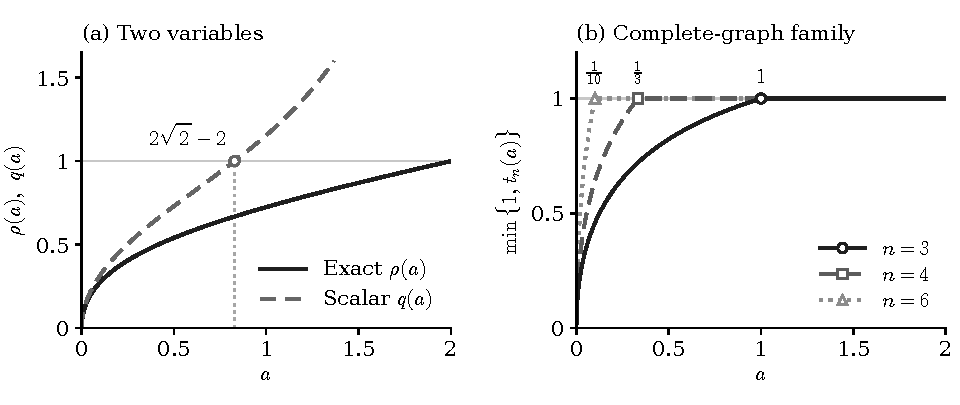
\includegraphics[width=\linewidth]{figures/rates}
\caption{Analytic Jacobi factors at $U=f^*=0$ for termwise McCormick
relaxations with exact square terms. (a) For $f=x^2+y^2+axy$, the exact
cube factor $\rho(a)$ is below one for $0<a<2$
(Proposition~\ref{prop:two-variable-rate}). The scalar quadratic-growth
bound with $\mu=1-a^2/4$ and $\tau=a/4$ gives
$q(a)=\sqrt{a/(1-a^2/4)}$; its sufficient condition $q<1$ holds only for
$a<2\sqrt2-2$ (Proposition~\ref{prop:quadratic-growth}). The scalar curve
is shown through $q=1.6$. (b) For
$f=\sum_i x_i^2+a\sum_{i<j}x_ix_j$, $n\ge3$, the exact cube factor
$\min\{1,t_n(a)\}$ reaches one at $a=2/[(n-1)(n-2)]$
(Example~\ref{ex:many-term}). Markers identify the thresholds $1$, $1/3$,
and $1/10$ for $n=3,4,6$. All objectives are strongly convex for $0<a<2$;
the plateaus denote fixed cubes at every scale. Endpoints show continuous
limits.}
\label{fig:analytic-rates}
\end{figure}

\begin{example}[The sign pattern matters]\label{ex:signed-stall}
Let $f=x_1^2+x_2^2+x_3^2+\tfrac34(x_1x_2+x_1x_3-x_2x_3)$ on $[-1,1]^3$. Its
Hessian $2I+\tfrac34A$ with $A=\left[\begin{smallmatrix}0&1&1\\1&0&-1\\1&-1&0\end{smallmatrix}\right]$
has eigenvalues $1/2,11/4,11/4$, because $(-1,1,1)$, $(0,1,-1)$, and
$(2,1,1)$ are eigenvectors of $A$ with eigenvalues $-2,1,1$. The row
condition fails in every row ($5/2>9/4$). By~\eqref{eq:cube-Q},
\[
  Q(1,\xi)=\norm{\xi}_2^2+\tfrac34\bigl(\abs{\xi_1+\xi_2}+\abs{\xi_1+\xi_3}
  +\abs{\xi_2-\xi_3}-3\bigr),
\]
and at $z=(1,-3/8,-3/8)$ the value is $41/32-18/32-24/32=-1/32$. The signed
permutations $(\xi_1,\xi_2,\xi_3)\mapsto(\xi_2,\xi_1,-\xi_3)$ and
$(\xi_1,\xi_2,\xi_3)\mapsto(\xi_3,-\xi_2,\xi_1)$ preserve the cube and
permute the three absolute values, so they preserve $Q(1,\cdot)$; they map
$z$ to points on the positive second and third faces, and $Q(1,-\xi)=Q(1,\xi)$
gives the negative faces. Theorem~\ref{thm:local-stall} applies with a strict
margin. For this objective, condition (b) of
Proposition~\ref{prop:quadratic-rows} gives the lower bound $-1/32$ on every
face value, which $z$ attains.
\end{example}

\begin{example}[The shape changes the outcome]\label{ex:shape-change}
Let $f=\sum_{i=1}^3x_i^2+\sum_{i<j}x_ix_j$, the case $a=1$, $n=3$ of
Example~\ref{ex:many-term}, for which the cube stalls with equality in the
row condition. On the thinner box $[-1/4,1/4]\times[-1,1]^2$, use the scaled
matrix $H'=\operatorname{diag}(1/4,1,1)\,H\,\operatorname{diag}(1/4,1,1)$. For
$k=1$, the witnesses $\pm e_1$ of part (a) of
Proposition~\ref{prop:quadratic-rows} give face values at most
$H'_{11}/2-S_1=1/16-1<0$. For $k=2,3$, the estimate in the proof of part (b),
which holds coordinate by coordinate, gives face values at least
$1-3/16-1/4-1/4=5/16>0$. Hence the first coordinate keeps its bounds and the
other two contract. A round changes the shape, and the face test must then
be applied to the new shape.
\end{example}

\begin{example}[Finite tangent relaxations of squares]\label{ex:finite-square}
Let $f=\sum_ix_i^2$ and relax each square $x_i^2$ by a lifted variable $y_i$
subject to the McCormick inequalities for the product $x_i\cdot x_i$, which
are the endpoint tangents $y_i\ge2\ell_ix_i-\ell_i^2$ and
$y_i\ge2u_ix_i-u_i^2$ and the secant $y_i\le(\ell_i+u_i)x_i-\ell_iu_i$; the
objective is $\sum_iy_i$. On a centered box with half-widths $h_i>0$,
$\phi_B(x)=\sum_i(2h_i\abs{x_i}-h_i^2)$, and a Jacobi round at $U=0$ gives
the exact map
\[
  h_i'=\min\Bigl\{h_i,\ \frac{1}{2h_i}\sum_jh_j^2\Bigr\}:
\]
the coordinates $j\ne i$ can be zero with $y_j=-h_j^2$, and the endpoint is
attained with these values. For $n=1$ the half-width halves each round. For
$n\ge2$ every cube is fixed, although the objective is strictly convex with
a unique minimizer; the tangent model is $Q(1,\xi)=\sum_i(2\abs{\xi_i}-1)$,
whose face values $2-n$ are nonpositive. Adding the valid rows $y_i\ge0$
changes the map to $h_i'=h_i/2$, and the exact convex squares give $\{0\}$
after one round. The rate is a property of the relaxation, not of the
problem. Section~\ref{sec:certificates} uses this finite family as its
exact reference family.
\end{example}

\subsection{Factorable functions and composite McCormick relaxations}\label{sec:local-rates-factorable}

For general smooth objectives the tangent model is computed by a recursion
over a factorable representation. A \emph{factorable representation} is a
sequence $v_1,\dots,v_m$ of functions of $x$ with $v_i=x_i$ for $i\le n$
and, for $k>n$, one of: a constant; $v_a+v_b$; $c\,v_a$ with $c\in\R$;
$v_av_b$ (with $a=b$ allowed); or $h_k(v_a)$ for a function $h_k$ of one
variable, where $a,b<k$. The objective is $f=v_m$. On a box $B$, natural
interval arithmetic gives intervals $[v_k^L(B),v_k^U(B)]$: endpoint
operations for sums and scalings, the minimum and maximum of the four
endpoint products for products, and the exact range of $h_k$ over the
interval of its argument for univariate factors. The composite McCormick
relaxation~\cite{mccormick1976-computability-of-global-solutions-to,mitsos2009-mccormick-based-relaxations-of-algorithms}
computes convex and concave relaxations $\mathrm{cv}_k\le v_k\le\mathrm{cc}_k$
on $B$ factor by factor: sums and scalings exactly (a negative scaling
exchanges the convex and concave sides); products by the rule
\begin{align*}
  \mathrm{cv}_k&=\max\bigl\{\alpha_1+\alpha_2-v_a^Lv_b^L,\ \beta_1+\beta_2-v_a^Uv_b^U\bigr\},\\
  \alpha_1&=\min\{v_b^L\mathrm{cv}_a,v_b^L\mathrm{cc}_a\},\quad
  \alpha_2=\min\{v_a^L\mathrm{cv}_b,v_a^L\mathrm{cc}_b\},\\
  \beta_1&=\min\{v_b^U\mathrm{cv}_a,v_b^U\mathrm{cc}_a\},\quad
  \beta_2=\min\{v_a^U\mathrm{cv}_b,v_a^U\mathrm{cc}_b\},
\end{align*}
and, with $\gamma_1=\max\{v_b^L\mathrm{cv}_a,v_b^L\mathrm{cc}_a\}$,
$\gamma_2=\max\{v_a^U\mathrm{cv}_b,v_a^U\mathrm{cc}_b\}$,
$\gamma_3=\max\{v_b^U\mathrm{cv}_a,v_b^U\mathrm{cc}_a\}$, and
$\gamma_4=\max\{v_a^L\mathrm{cv}_b,v_a^L\mathrm{cc}_b\}$,
\[
  \mathrm{cc}_k=\min\bigl\{\gamma_1+\gamma_2-v_a^Uv_b^L,\ \gamma_3+\gamma_4-v_a^Lv_b^U\bigr\};
\]
univariate factors are relaxed by
$\mathrm{cv}_k=h^{\mathrm{cv}}_Z(\midop\{\mathrm{cv}_a,\mathrm{cc}_a,z^{\min}\})$,
where $h^{\mathrm{cv}}_Z$ is the convex envelope of $h_k$ on
$Z=[v_a^L,v_a^U]$, $z^{\min}$ is a minimizer of $h^{\mathrm{cv}}_Z$ on $Z$, and
$\midop$ is the median of three numbers; the concave side uses the concave
envelope and a maximizer. The relaxed objective is
$\phi_B=\mathrm{cv}_m$. The \emph{clipped} variant replaces $\mathrm{cv}_k$ by
$\max\{\mathrm{cv}_k,v_k^L\}$ and $\mathrm{cc}_k$ by $\min\{\mathrm{cc}_k,v_k^U\}$
before they are used by later factors. Scott, Stuber, and Barton prove that
the clipped construction is monotone in the sense of~\eqref{eq:monotonicity}
when the natural interval of every univariate argument lies in the domain
of the corresponding scalar function and these functions are Lipschitz
there, and they note that the unclipped rule can violate
monotonicity~\cite{scott2011-generalized-mccormick-relaxations}. On small
boxes around a point at which the scalar functions are twice continuously
differentiable, these conditions hold. Validity and convexity of both
variants are standard.

The tangent model is built from first-order data. Write $v_k^*=v_k(x^*)$
and $\pi_k(\xi)=\nabla v_k(x^*)^T\xi$, and, for $t\in\R$,
$t^+=\max\{t,0\}$ and $t^-=\max\{-t,0\}$. For a shape $d$ define intervals
$[\underline\pi_k(d),\overline\pi_k(d)]$ and nonnegative functions
$E_k^{\mathrm{cv}}(d,\xi)$, $E_k^{\mathrm{cc}}(d,\xi)$, $\xi\in D(d)$, by the
following recursion.
\begin{itemize}
\item Variable $x_i$: interval $[-d_i^-,d_i^+]$, $E^{\mathrm{cv}}=E^{\mathrm{cc}}=0$.
  Constant: interval $[0,0]$, $E^{\mathrm{cv}}=E^{\mathrm{cc}}=0$.
\item Sum: intervals and both functions add.
\item Scaling $c\,v_a$: for $c\ge0$, interval $c[\underline\pi_a,\overline\pi_a]$,
  $E^{\mathrm{cv}}=cE_a^{\mathrm{cv}}$, $E^{\mathrm{cc}}=cE_a^{\mathrm{cc}}$; for
  $c<0$, interval $[c\overline\pi_a,c\underline\pi_a]$,
  $E^{\mathrm{cv}}=\abs cE_a^{\mathrm{cc}}$, $E^{\mathrm{cc}}=\abs cE_a^{\mathrm{cv}}$.
\item Product $v_av_b$: interval
  $v_b^*[\underline\pi_a,\overline\pi_a]+v_a^*[\underline\pi_b,\overline\pi_b]$
  in interval arithmetic, and
  \begin{align*}
    E^{\mathrm{cv}}&=(v_b^*)^+E_a^{\mathrm{cv}}+(v_b^*)^-E_a^{\mathrm{cc}}
      +(v_a^*)^+E_b^{\mathrm{cv}}+(v_a^*)^-E_b^{\mathrm{cc}}\\
      &\quad+\min\bigl\{(\pi_a-\underline\pi_a)(\pi_b-\underline\pi_b),\
      (\overline\pi_a-\pi_a)(\overline\pi_b-\pi_b)\bigr\},\\
    E^{\mathrm{cc}}&=(v_b^*)^+E_a^{\mathrm{cc}}+(v_b^*)^-E_a^{\mathrm{cv}}
      +(v_a^*)^+E_b^{\mathrm{cc}}+(v_a^*)^-E_b^{\mathrm{cv}}\\
      &\quad+\min\bigl\{(\overline\pi_a-\pi_a)(\pi_b-\underline\pi_b),\
      (\pi_a-\underline\pi_a)(\overline\pi_b-\pi_b)\bigr\}.
  \end{align*}
\item Univariate $h_k(v_a)$, with $h_1=h_k'(v_a^*)$, $h_2=h_k''(v_a^*)$, and
  $\sigma_a=(\pi_a-\underline\pi_a)(\overline\pi_a-\pi_a)$: interval
  $h_1[\underline\pi_a,\overline\pi_a]$, and
  \[
    E^{\mathrm{cv}}=\tfrac12h_2^-\sigma_a+h_1^+E_a^{\mathrm{cv}}+h_1^-E_a^{\mathrm{cc}},\qquad
    E^{\mathrm{cc}}=\tfrac12h_2^+\sigma_a+h_1^+E_a^{\mathrm{cc}}+h_1^-E_a^{\mathrm{cv}}.
  \]
\end{itemize}
Here $\pi_a$ stands for $\pi_a(\xi)$ and the interval endpoints for their
values at $d$. The interval $[\underline\pi_k(d),\overline\pi_k(d)]$ is
natural interval arithmetic applied to the linearized factor sequence over
$D(d)$, so it contains $\pi_k(\xi)$ for $\xi\in D(d)$; consequently every
factor of the form $\pi-\underline\pi$ or $\overline\pi-\pi$ is nonnegative
and $E_k^{\mathrm{cv}},E_k^{\mathrm{cc}}\ge0$. By induction, the interval
endpoints are continuous and positively homogeneous of degree one in $d$,
and the functions $E_k$ are continuous and positively homogeneous of degree
two in $(d,\xi)$.

\begin{theorem}[Second-order expansion of composite McCormick relaxations]\label{thm:composite-expansion}
Let $x^*\in\R^n$, and suppose that for every univariate factor
$v_k=h_k(v_a)$, the function $h_k$ is twice continuously differentiable on
an open interval containing $v_a(x^*)$. Let $\mathcal K$ be a compact set of
shapes. There is $t_{\mathcal K}>0$ such that for $0<t\le t_{\mathcal K}$ all
intervals and relaxations on $B_t=x^*+tD(d)$, $d\in\mathcal K$, are defined,
and, uniformly over $d\in\mathcal K$ and $\xi\in D(d)$, with $x_t=x^*+t\xi$,
for every factor $k$,
\begin{align}
  v_k^L(B_t)&=v_k^*+t\underline\pi_k(d)+O(t^2),\qquad
  v_k^U(B_t)=v_k^*+t\overline\pi_k(d)+O(t^2),\label{eq:expansion-interval}\\
  \mathrm{cv}_k(x_t)&=v_k(x_t)-t^2E_k^{\mathrm{cv}}(d,\xi)+o(t^2),\qquad
  \mathrm{cc}_k(x_t)=v_k(x_t)+t^2E_k^{\mathrm{cc}}(d,\xi)+o(t^2),\label{eq:expansion-relaxation}\\
  v_k^L(B_t)&-\mathrm{cv}_k(x_t)\le o(t^2),\qquad
  \mathrm{cc}_k(x_t)-v_k^U(B_t)\le o(t^2),\label{eq:expansion-dominance}
\end{align}
where the relaxations are those built on $B_t$. If each $h_k''$ is
Lipschitz near $v_a(x^*)$, every $o(t^2)$ can be replaced by $O(t^3)$. The
clipped relaxations have the same expansions. Consequently,
\[
  \phi_{B_t}(x_t)=f(x^*)+t\nabla f(x^*)^T\xi+t^2Q(d,\xi)+o(t^2),\qquad
  Q(d,\xi)=\tfrac12\xi^T\nabla^2f(x^*)\xi-E_m^{\mathrm{cv}}(d,\xi),
\]
uniformly on $\mathcal K$, and $Q$ is continuous. At a minimizer with
$\nabla f(x^*)=0$ at which the relaxations are monotone, for example in
the clipped construction, Assumption~\ref{ass:tangent} holds.
\end{theorem}

The proof is in Appendix~\ref{sec:local-proofs-composite}. Its main step
concerns univariate factors: the median rule can clip the argument of the
envelope at an endpoint of its interval, and~\eqref{eq:expansion-dominance}
shows that this clipping does not change the second-order term. The
expansion covers zero factor values, critical points $h_k'(v_a^*)=0$,
inflection points $h_k''(v_a^*)=0$, first-order intervals of zero width,
and shapes with zero components. The box $B_0$ plays no role, so the
theorem also applies at minimizers on the boundary of $B_0$, with shapes
restricted to the admissible ones; this is used in
Section~\ref{sec:local-rates-boundary}. The smoothness hypothesis concerns
each scalar factor at its own argument, and smoothness of $f$ does not
replace it. For example, $f(x)=\abs x-\abs x+x^2=x^2$, with the square kept
exact, has on $[-t,t]$ the composite relaxation $x^2+\abs x-t$, with or
without clipping: the concave envelope of $\abs x$ is the constant $t$, and
the subtraction uses it. The gap at $x^*=0$ is $t$, of first order. The
direct relaxation of $\abs x$ itself is exact, so nonsmoothness alone does
not force such an error; the theorem simply does not apply at a kink. At a
nonzero argument, $\abs{\cdot}$ is linear nearby and the theorem applies.

Two consequences are worth stating. First, for quadratic objectives with
the squares represented as univariate factors and the products of distinct
variables as products, $E_m^{\mathrm{cv}}$ is the McCormick gap and
Theorem~\ref{thm:composite-expansion} reproduces~\eqref{eq:quadratic-Q}.
Representing $x_i^2$ instead as the product $x_i\cdot x_i$ gives, at
$x_i^*=0$, the gap $\min\{(\xi_i+d_i^-)^2,(d_i^+-\xi_i)^2\}$ and the model
$2\abs{\xi_i}-1$ on the unit interval, which is the finite tangent
relaxation of Example~\ref{ex:finite-square}. The tangent model therefore
depends on the factorable representation as well as on the rules. Second,
since $E_m^{\mathrm{cv}}$ is bounded on compact sets, the theorem gives
$\phi_B\ge f-Cw(B)^2$ on small boxes containing $x^*$. This recovers, near
$x^*$, the second-order pointwise convergence of McCormick
relaxations~\cite{bompadre2012-convergence-rate-of-mccormick-relaxations}; the theorem
adds the limit of the scaled gap as a function of the box shape and of the
position in the box, which is what the tangent map needs.

Solvers usually relax lifted reformulations with an auxiliary variable per
factor. For quadratic problems whose auxiliary variables occur only in the
objective, minimizing over the auxiliaries decouples the terms. With exact
convex squares and McCormick envelopes for the products of distinct
variables, this yields the termwise relaxation, so~\eqref{eq:quadratic-Q}
applies exactly; with finite tangent relaxations of the squares it yields
the model of Example~\ref{ex:finite-square}. When
auxiliary variables also occur in constraints, or when cuts are added,
Theorem~\ref{thm:composite-expansion} does not apply, and
Assumption~\ref{ass:tangent} is a hypothesis to be verified for the
construction at hand.

\subsection{Minimizers on the boundary of the box}\label{sec:local-rates-boundary}

At a minimizer on the boundary of $B_0$ with nonzero derivatives across the
active faces, the first-order term dominates in the active coordinates.
Let $x^*$ be a global minimizer with $x_i^*=\ell_i^0$ for $i$ in an active
set $A$ and $\ell_i^0<x_i^*<u_i^0$ for $i$ in the free set $F$; active upper
bounds reduce to this case by reflecting the coordinate. We assume that $A$ and $F$ are both nonempty; the case $F=\emptyset$ is
discussed after Theorem~\ref{thm:boundary}. Let $g\in\R^n$ satisfy $g_i>0$
for $i\in A$ and $g_i=0$ for $i\in F$. For a differentiable objective with
$g=\nabla f(x^*)$ and no constraints other than the bounds, these are the
first-order optimality conditions with strict complementarity; with other
constraints, $g$ is the first-order coefficient of the projected
relaxation in Assumption~\ref{ass:boundary} below. Admissible shapes form the closed cone
$\mathcal S=\{d\ge0:d_i^-=0\text{ for }i\in A\}$; every box $B$ with
$x^*\in B\subseteq B_0$ equals $x^*+tD(d)$ with $d\in\mathcal S$. Write
$w_i(B)=u_i-\ell_i$ for the width of coordinate $i$.

\begin{assumption}[Boundary tangent model]\label{ass:boundary}
There is a continuous function $Q(d,\xi)$ on
$\{(d,\xi):d\in\mathcal S,\ \xi\in D(d)\}$ such that for every compact
$\mathcal K\subseteq\mathcal S$ the comparison boxes belong to $\mathfrak B$
for small $t$ and
\[
  \varrho_{\mathcal K}(t)=\sup_{d\in\mathcal K,\ \xi\in D(d)}
  \frac{\bigl|\phi_{x^*+tD(d)}(x^*+t\xi)-f^*-tg^T\xi-t^2Q(d,\xi)\bigr|}{t^2}
  \longrightarrow0.
\]
\end{assumption}

The essential point is that $\mathcal K$ may contain shapes whose active
components are zero or small. Theorem~\ref{thm:composite-expansion}
supplies Assumption~\ref{ass:boundary} for clipped composite McCormick
relaxations with $g=\nabla f(x^*)$. For a free shape $d_F$ let $\iota(d_F)$ be
the shape with free part $d_F$ and zero active components, define $\iota$
on points in the same way, and set
\[
  Q^F(d_F,\xi_F)=Q(\iota(d_F),\iota(\xi_F)),\qquad
  G^F(d_F)=-\min_{\xi_F\in D_F(d_F)}Q^F(d_F,\xi_F)\ge0.
\]
The reduced tangent map $\Phi^F_c$ and its factor $r^*(\Phi^F)$ are defined
from $Q^F$ as in Section~\ref{sec:local-rates-tangent}. For the boundary
theorem fix a free shape $u_F\gg0$ and a bound $M\ge0$ on the initial
active components, and let
\[
  G_0=G^F(u_F),\qquad
  G_M=-\min\{Q(d,\xi):d\in\mathcal S,\ d_F=u_F,\ d_A^+\le M,\ \xi\in D(d)\},
  \qquad g_{\min}=\min_{i\in A}g_i.
\]
Since $\iota(u_F)$ is admissible, $0\le G_0\le G_M$.

\begin{lemma}[One round near a boundary minimizer]\label{lem:boundary-step}
Let Assumption~\ref{ass:boundary} hold, let $\delta>0$, and let $\mathcal K_F$
be a compact set of free shapes. There are $\bar t,\bar\sigma>0$ such that
for every box $B=x^*+tD(d)$ with $d\in\mathcal S$, $d_F\in\mathcal K_F$,
$\max_{i\in A}d_i^+\le\bar\sigma$, and $t\le\bar t$, and every $\epsilon\ge0$:
\begin{enumerate}[label=(\roman*)]
\item if $\epsilon\le\delta t^2/2$, the free part of $T_U(B)$ lies in
  $x_F^*+tD_F(\Phi^F_\delta(d_F))$;
\item $x^*+t\iota(\xi_F)\in K_U(B)$ for every $\xi_F\in D_F(d_F)$ with
  $Q^F(d_F,\xi_F)\le-\delta$;
\item $w_i(T_U(B))\le\bigl(\epsilon+(G^F(d_F)+\delta/2)t^2\bigr)/g_i$ for
  $i\in A$;
\item $w_i(T_U(B))\ge\min\bigl\{td_i^+,\ \bigl(\epsilon+(G^F(d_F)-\delta/2)t^2\bigr)/g_i\bigr\}$
  for $i\in A$.
\end{enumerate}
\end{lemma}

Parts (i) and (ii) say that in scaled coordinates the free part of one
round lies between the hulls of the sublevel sets of $Q^F$ at levels
$-\delta$ and $\delta$. Parts (iii) and (iv) show that the bound on the active
widths is sharp to first order, since $\delta$ is arbitrary. The proof is
in Appendix~\ref{sec:local-proofs-boundary}.

\begin{theorem}[Boundary minimizers]\label{thm:boundary}
Let Assumption~\ref{ass:boundary} hold, and let $u_F\gg0$, $\delta>0$, and
$\lambda\in(0,1)$ satisfy $\Phi^F_\delta(u_F)\le\lambda u_F$. Let $M\ge0$.
There is $\bar t>0$ with the following property. Let the start box satisfy
$x^*\in B_0\subseteq x^*+t_0D(d^0)$ with an admissible shape
$d^0\in\mathcal S$, $d^0_F=u_F$, $\max_{i\in A}(d^0)_i^+\le M$, and
$0<t_0\le\bar t$, and consider Jacobi iterates, or complete sequential
rounds, from $B_0$ at cutoff $U=f^*+\epsilon$. Put $t_k=\lambda^{k-1}t_0$ for $k\ge1$, and let
$N=\min\{k\ge1:t_k^2<2\epsilon/\delta\}$, with $N=\infty$ if $\epsilon=0$.
\begin{enumerate}[label=(\alph*)]
\item For $1\le k\le N$, the free part of $B_k$ lies in
  $x_F^*+t_kD_F(u_F)$.
\item $w_i(B_1)\le\bigl(\epsilon+(G_M+\delta/4)t_0^2\bigr)/g_i$ for $i\in A$. If
  $N\ge2$, then for $1\le k\le N$ and $i\in A$,
  \[
    w_i(B_{k+1})\le\bigl(\epsilon+(G_0+\eta_k)t_k^2\bigr)/g_i,
  \]
  with $0\le\eta_k\le\delta/2$, and $\eta_k\to0$ as $t_k\to0$.
\item If $\epsilon=0$, then $B_\infty=\{x^*\}$, the free widths are
  $O(\lambda^k)$ by (a), and $w_i(B_{k+1})\le(G_0/g_i+o(1))\,t_k^2$. If $\epsilon>0$, the free part of
  $B_\infty$ lies in $x_F^*+\sqrt{2\epsilon/\delta}\,D_F(u_F)$ and
  $w_i(B_\infty)\le(2+2G_M/\delta)\,\epsilon/g_i$ for $i\in A$.
\end{enumerate}
Every $\lambda>r^*(\Phi^F)$ admits such $u_F$ and $\delta$.
\end{theorem}

The free coordinates thus obey the upper bounds of the interior theory,
with the reduced map $\Phi^F$ and a floor of order at most $\sqrt\epsilon$,
while the active widths are at most of order $\epsilon$ plus the square of
the free scale $t_k$. The statement bounds the free parts and the active
widths by the common geometric scale $t_k$; it does not assert that the
actual free gauge contracts in every round. It need not: for $f=x+y^2$ on
$x\ge0$ with the valid monotone family $\phi_B=f-h^2$, where $h$ is the
upper extent of $B$ in $x$, a Jacobi round at zero cutoff maps the active
extent $h$ to $\min\{h,h^2\}$ and the free radius $r$ to $\min\{r,h\}$, so from
$[0,t_0]\times[-t_0^3,t_0^3]$ with $0<t_0<1$ the free radius does not move in
the first two rounds. The proof is in Appendix~\ref{sec:local-proofs-boundary}. If
$g_i=0$ for some active $i$, that coordinate has no first-order term. It
can be treated as a free coordinate restricted to shapes with $d_i^-=0$:
the same proof applies to the enlarged free set, provided the contraction
hypothesis $\Phi^F_\delta(u_F)\le\lambda u_F$ is verified on this one-sided
cone of shapes. If all coordinates are active ($F=\emptyset$) with
$g_i>0$, Proposition~\ref{prop:sharp-growth} applies on small boxes: at zero
cutoff slack the convergence is quadratic, and at a positive slack the
widths satisfy the forced recurrence of that proposition and end at most
$4\epsilon/\kappa$.

The refined estimate in (b) requires $N\ge2$. If the initial scale already
lies below the cutoff floor, the active components of $B_1$ need not be
small relative to $t_1$, and the refined constant can fail. For
$f(x,y)=x-x^2+y^2$ on $[0,1/4]\times[-1/4,1/4]$, keep $y^2$ exact and use the
secant $-hx$ of $-x^2$ on $[0,h]$. On $B=[0,h]\times[-r,r]$ the relaxation is
$(1-h)x+y^2$; the expansion is exact with $g=(1,0)$ and
$Q(d,\xi)=-d_x^+\xi_x+\xi_y^2$, so $G_0=0$, and $u_F=1$, $\delta=1/4$,
$\lambda=3/4$, $M=1$ satisfy the hypotheses. Start from
$[0,w_0]\times[-w_0,w_0]$ with $\epsilon=w_0/2$ and $w_0$ small. Then $N=1$,
the free bounds do not move in the first two rounds, and the active widths
are $h_1=\epsilon/(1-w_0)$ and $h_2=\epsilon/(1-h_1)$. Hence
$(h_2-\epsilon)/w_0^2=1/(4-6w_0)>1/4$, whereas the refined estimate would give
at most $\delta/2=1/8$.

\begin{example}[An exact boundary example]\label{ex:boundary}
Let $f=x_1+x_2^2+x_3^2+ax_2x_3$ with $0<a<2$ on $[0,1]\times[-1,1]^2$, with
exact squares and the McCormick underestimator of $x_2x_3$. The minimizer
is $0$, with $A=\{1\}$, $g_1=1$, and $G_0=a$. On $B=[0,h]\times[-s,s]^2$ the
relaxation is $x_1+\psi_s(x_2,x_3)$ with
$\psi_s=x_2^2+x_3^2+as\abs{x_2+x_3}-as^2$, whose minimum is $-as^2$. A Jacobi
round at cutoff $\epsilon$ therefore maps $(h,s)$ to
\[
  \bigl(\min\{h,\ \epsilon+as^2\},\ g(s)\bigr),
\]
with $g$ as in Proposition~\ref{prop:two-variable-cutoff-floor}: the
largest free extent is attained with $x_1=0$, and the largest active extent
with $(x_2,x_3)=0$. For $\epsilon=0$ the free half-width is $\rho(a)^ks_0$ and
the active width is $a\rho(a)^{2k-2}s_0^2$ once it falls below $h_0$. For
$\epsilon>0$ and $s_0\ge h_\epsilon$, the free half-width decreases to
$h_\epsilon$ and the active width to
$\min\{h_0,\ \epsilon(1+a/(1-a^2/4))\}$: a free floor of order $\sqrt\epsilon$
and an active floor of order $\epsilon$. For $a=1$ the limit widths are
$2h_\epsilon=(4/\sqrt3)\sqrt\epsilon\approx2.309\sqrt\epsilon$ and, for large
$h_0$, $7\epsilon/3$.
\end{example}

\subsection{The relaxation gap after tightening, and stopping}\label{sec:local-rates-consequences}

The width of the limit box matters because it controls the relaxation gap
that remains after tightening.

\begin{corollary}[Gap after tightening]\label{cor:local-gap}
Under the hypotheses of Theorem~\ref{thm:tangent-contraction}(b), let
\[
  G=-\min_{\xi\in D(u)}Q(u,\xi)\ge0.
\]
If $\epsilon>0$ and $\sqrt{2\epsilon/\delta}\le\bar t$, then
\[
  f^*-L(B_\infty)\le\Bigl(\frac{2G}{\delta}+1\Bigr)\epsilon,
\]
and $f^*-L(B_\infty)\le(2G/\delta)\epsilon+o(\epsilon)$ as $\epsilon\downarrow0$;
for $\epsilon=0$, $L(B_\infty)=f^*$. Under the hypotheses of
Proposition~\ref{prop:sharp-growth}, once an iterate has width at most
$\kappa/(4\tau)$ (any iterate if $\tau=0$),
$f^*-L(B_\infty)\le16\tau\epsilon^2/\kappa^2$.
\end{corollary}

\begin{proof}
Let $t_\epsilon=\sqrt{2\epsilon/\delta}$ and $C=x^*+t_\epsilon D(u)$. By
Theorem~\ref{thm:tangent-contraction}, $B_\infty\subseteq C$, so $L(B_\infty)\ge L(C)$.
For $x=x^*+t_\epsilon\xi\in C$,
$\phi_C(x)\ge f^*+t_\epsilon^2Q(u,\xi)-\varrho_{\{u\}}(t_\epsilon)t_\epsilon^2
\ge f^*-Gt_\epsilon^2-\varrho_{\{u\}}(t_\epsilon)t_\epsilon^2$. Since
$\varrho_{\{u\}}(t_\epsilon)\le\delta/2$, this gives the first bound, and since
$\varrho_{\{u\}}(t_\epsilon)\to0$, the second. For $\epsilon=0$,
$B_\infty=\{x^*\}$ lies in every comparison box, so the same estimate with
$t\downarrow0$ gives $L(B_\infty)\ge f^*$, and validity at $x^*$ gives equality.
In the sharp case,~\eqref{eq:sharp-growth} gives $L(B)\ge f^*-\tau w(B)^2$
for boxes containing $x^*$, and $w(B_\infty)\le4\epsilon/\kappa$.
\end{proof}

Under the contraction hypotheses, the gap left after tightening to the
limit is at most proportional to the incumbent's suboptimality $\epsilon$;
for the model problem it equals $a\epsilon/(1-a^2/4)$
(Proposition~\ref{prop:two-variable-cutoff-floor}). Together with the
$O(\sqrt\epsilon)$ bound on the width, this has several consequences for
deciding when to tighten.

\paragraph{Rounds to the cutoff floor.} Under the hypotheses of
Theorem~\ref{thm:tangent-contraction}, the gauge falls at least by the
factor $\lambda$ per round until it is below $\sqrt{2\epsilon/\delta}$.
For $\epsilon>0$, zero rounds suffice when the starting gauge satisfies
$t_0\le\sqrt{2\epsilon/\delta}$. Otherwise at most
$\bigl\lceil\log\bigl(t_0\sqrt{\delta/(2\epsilon)}\bigr)/\log(1/\lambda)\bigr\rceil$
rounds bring the iterates inside $x^*+\sqrt{2\epsilon/\delta}\,D(u)$, which
contains the limit; further rounds change the box only inside this region
and change the gap by at most the $O(\epsilon)$ bound above. This bound on
the number of rounds grows only logarithmically as $\epsilon$ decreases.

\paragraph{When to repeat after an incumbent improves.} Lowering the
cutoff slack from $\epsilon$ to $\epsilon'$ lowers the bounds on the limit
width by the factor $\sqrt{\epsilon'/\epsilon}$ and the bounds on the remaining
gap by the factor $\epsilon'/\epsilon$; in the model problem the limit itself
shrinks by exactly these factors. This is the local reason to repeat
tightening after an incumbent improves, and the reason why a cutoff far
above $f^*$ limits the value of any number of rounds. In the stall regime
of Theorem~\ref{thm:local-stall}, by contrast, no improvement of the
incumbent removes the fixed boxes around $x^*$.

\paragraph{What observed ratios show.} The successive width ratios of an
iteration are a natural signal for stopping, and they estimate the
contraction rate in favorable cases. They are not a certificate. From boxes
that are not eigenvectors, early ratios can lie far below the asymptotic
rate (the example after Proposition~\ref{prop:rectangle-map});
near a positive floor the ratios tend to one while the distance to the
limit contracts quickly (Proposition~\ref{prop:two-variable-cutoff-floor}(d));
a ratio near one can thus indicate a rate near one, the approach to a floor,
or a stall. Example~\ref{ex:critical-scalar} has ratios tending to one and still
converges to a point, sublinearly. Proposition~\ref{prop:history} gives valid
monotone relaxation families whose iterations share arbitrarily long
histories and then either stall or contract to a point. Observed ratios
therefore support stopping heuristics, not guarantees.

\paragraph{Which regimes admit finite certificates.} In the stall regime,
the witnesses of Theorem~\ref{thm:local-stall} are finitely many points
whose coordinate hull is a fixed box at every small scale; they are a
certificate of the kind developed in Section~\ref{sec:certificates}. In the
contracting regime with $\epsilon>0$, the limit box is a fixed box of width
$O(\sqrt\epsilon)$ under~\eqref{eq:closed-family}, and $2n$ points
attaining its faces certify it, as in
Proposition~\ref{prop:two-variable-cutoff-floor}(b). In the contracting
regime with $\epsilon=0$, the only fixed box containing $x^*$ in a small
neighborhood is $\{x^*\}$; no box of positive width can certify that the
remaining movement is zero. An iterate that reaches $\{x^*\}$ can be
certified as fixed. If convergence is only asymptotic, as in the model
problem, a bound on the remaining movement, such as the residual certificate
of Section~\ref{sec:residual}, justifies a tolerance stop. When the optimal
incumbent lies in the current box, its protected singleton
(Corollary~\ref{cor:original-points}) already bounds the remaining movement,
and the bound is exact if the iterates converge to it.
These cases do not exhaust the possibilities:
Example~\ref{ex:critical-scalar} has no fixed box of positive width and no
geometric contraction.

\paragraph{Symmetry and spread minimizers.} By Lemma~\ref{lem:sublevel-hull},
several global minimizers keep their hull in every iterate, whatever the
local rates. Tightening at the root of a symmetric model cannot converge to a single
point until branching separates the minimizers. At a node that contains a
single minimizer, the conclusions of this section apply when their
hypotheses hold: a tangent model, monotonicity on the comparison boxes, a
contraction shape, and a start box in the local region. A single minimizer
does not supply them; Example~\ref{ex:many-term} has a unique minimizer and
stalls.
